\documentclass[11pt]{article}\usepackage[]{graphicx}\usepackage[]{color}
%% maxwidth is the original width if it is less than linewidth
%% otherwise use linewidth (to make sure the graphics do not exceed the margin)
\makeatletter
\def\maxwidth{ %
  \ifdim\Gin@nat@width>\linewidth
    \linewidth
  \else
    \Gin@nat@width
  \fi
}
\makeatother

\definecolor{fgcolor}{rgb}{0.345, 0.345, 0.345}
\newcommand{\hlnum}[1]{\textcolor[rgb]{0.686,0.059,0.569}{#1}}%
\newcommand{\hlstr}[1]{\textcolor[rgb]{0.192,0.494,0.8}{#1}}%
\newcommand{\hlcom}[1]{\textcolor[rgb]{0.678,0.584,0.686}{\textit{#1}}}%
\newcommand{\hlopt}[1]{\textcolor[rgb]{0,0,0}{#1}}%
\newcommand{\hlstd}[1]{\textcolor[rgb]{0.345,0.345,0.345}{#1}}%
\newcommand{\hlkwa}[1]{\textcolor[rgb]{0.161,0.373,0.58}{\textbf{#1}}}%
\newcommand{\hlkwb}[1]{\textcolor[rgb]{0.69,0.353,0.396}{#1}}%
\newcommand{\hlkwc}[1]{\textcolor[rgb]{0.333,0.667,0.333}{#1}}%
\newcommand{\hlkwd}[1]{\textcolor[rgb]{0.737,0.353,0.396}{\textbf{#1}}}%

\usepackage{framed}
\makeatletter
\newenvironment{kframe}{%
 \def\at@end@of@kframe{}%
 \ifinner\ifhmode%
  \def\at@end@of@kframe{\end{minipage}}%
  \begin{minipage}{\columnwidth}%
 \fi\fi%
 \def\FrameCommand##1{\hskip\@totalleftmargin \hskip-\fboxsep
 \colorbox{shadecolor}{##1}\hskip-\fboxsep
     % There is no \\@totalrightmargin, so:
     \hskip-\linewidth \hskip-\@totalleftmargin \hskip\columnwidth}%
 \MakeFramed {\advance\hsize-\width
   \@totalleftmargin\z@ \linewidth\hsize
   \@setminipage}}%
 {\par\unskip\endMakeFramed%
 \at@end@of@kframe}
\makeatother

\definecolor{shadecolor}{rgb}{.97, .97, .97}
\definecolor{messagecolor}{rgb}{0, 0, 0}
\definecolor{warningcolor}{rgb}{1, 0, 1}
\definecolor{errorcolor}{rgb}{1, 0, 0}
\newenvironment{knitrout}{}{} % an empty environment to be redefined in TeX

\usepackage{alltt}
\usepackage{amsmath}
\usepackage{stmaryrd}
\usepackage{bbm}
\usepackage{amsmath}
\usepackage{mathtools}
\usepackage{pdfpages}

\newcount\colveccount
\newcommand*\colvec[1]{
        \global\colveccount#1
        \begin{pmatrix}
        \colvecnext
}
\def\colvecnext#1{
        #1
        \global\advance\colveccount-1
        \ifnum\colveccount>0
                \\
                \expandafter\colvecnext
        \else
                \end{pmatrix}
        \fi
}
\newcommand{\argmin}{\arg\!\min}

\author{Thibault Doutre, Student ID 26980469}
\title{STAT230 HW 2 \\
University of California, Berkeley}
\date{\today}
\IfFileExists{upquote.sty}{\usepackage{upquote}}{}
\begin{document}
\maketitle


\section{} 

\begin{knitrout}
\definecolor{shadecolor}{rgb}{0.969, 0.969, 0.969}\color{fgcolor}\begin{kframe}
\begin{alltt}
\hlkwd{load}\hlstd{(}\hlstr{'family.rda'}\hlstd{)}
\hlkwd{attach}\hlstd{(family)}
\end{alltt}
\end{kframe}
\end{knitrout}

 
\begin{knitrout}
\definecolor{shadecolor}{rgb}{0.969, 0.969, 0.969}\color{fgcolor}\begin{kframe}
\begin{alltt}
\hlstd{intercept} \hlkwb{=} \hlkwd{rep}\hlstd{(}\hlnum{1}\hlstd{,}\hlkwd{length}\hlstd{(weight))}
\hlstd{X} \hlkwb{=} \hlkwd{cbind}\hlstd{(intercept,height, bmi)}
\hlstd{betahat} \hlkwb{=} \hlkwd{solve}\hlstd{(}\hlkwd{crossprod}\hlstd{(X,X),} \hlkwd{t}\hlstd{(X)} \hlopt \hlstd{weight)}
\hlstd{betahat}
\end{alltt}
\begin{verbatim}
##                  [,1]
## intercept -310.346943
## height       4.675473
## bmi          6.308645
\end{verbatim}
\begin{alltt}
\hlstd{residuals} \hlkwb{=} \hlstd{weight} \hlopt{-} \hlstd{X} \hlopt \hlstd{betahat}
\hlstd{residuals}
\end{alltt}
\begin{verbatim}
##               [,1]
##  [1,] -0.676730632
##  [2,]  0.474100055
##  [3,] -0.264728345
##  [4,] -1.371495045
##  [5,]  2.176912620
##  [6,] -0.219261947
##  [7,] -0.413102763
##  [8,] -0.007851258
##  [9,] -0.800784395
## [10,]  3.819187100
## [11,] -1.272889595
## [12,] -1.086205171
## [13,] -1.289915027
## [14,]  0.932764403
\end{verbatim}
\end{kframe}
\end{knitrout}

\section{} 
\begin{knitrout}
\definecolor{shadecolor}{rgb}{0.969, 0.969, 0.969}\color{fgcolor}\begin{kframe}
\begin{alltt}
\hlstd{regcoef} \hlkwb{=} \hlkwa{function}\hlstd{(}\hlkwc{df}\hlstd{=family[}\hlnum{4}\hlopt{:}\hlnum{5}\hlstd{])\{}
  \hlstd{x} \hlkwb{=} \hlstd{df[,}\hlnum{1}\hlstd{]}
  \hlstd{y} \hlkwb{=} \hlstd{df[,}\hlnum{2}\hlstd{]}
  \hlstd{b} \hlkwb{=} \hlkwd{sum}\hlstd{((y}\hlopt{-}\hlkwd{mean}\hlstd{(y))}\hlopt{*}\hlstd{(x}\hlopt{-}\hlkwd{mean}\hlstd{(x)))}\hlopt{/}\hlkwd{sum}\hlstd{((x}\hlopt{-}\hlkwd{mean}\hlstd{(x))}\hlopt{^}\hlnum{2}\hlstd{)}
  \hlstd{a} \hlkwb{=} \hlkwd{mean}\hlstd{(y)} \hlopt{-} \hlstd{b}\hlopt{*}\hlkwd{mean}\hlstd{(x)}
  \hlkwd{return}\hlstd{(}\hlkwd{c}\hlstd{(a,b))}
\hlstd{\}}
\hlstd{regline} \hlkwb{=} \hlkwa{function}\hlstd{(}\hlkwc{df}\hlstd{=family[}\hlnum{4}\hlopt{:}\hlnum{5}\hlstd{])\{}
  \hlstd{coeff} \hlkwb{=} \hlkwd{regcoef}\hlstd{(df)}
  \hlkwd{plot}\hlstd{(height,weight,} \hlkwc{main} \hlstd{=} \hlstr{"Least Squares Regression Line"}\hlstd{,}
       \hlkwc{cex} \hlstd{= bmi}\hlopt{*}\hlnum{0.06}\hlstd{)}
  \hlkwd{abline}\hlstd{(coeff[}\hlnum{1}\hlstd{],coeff[}\hlnum{2}\hlstd{])}
\hlstd{\}}
\hlkwd{regline}\hlstd{()}
\end{alltt}
\end{kframe}
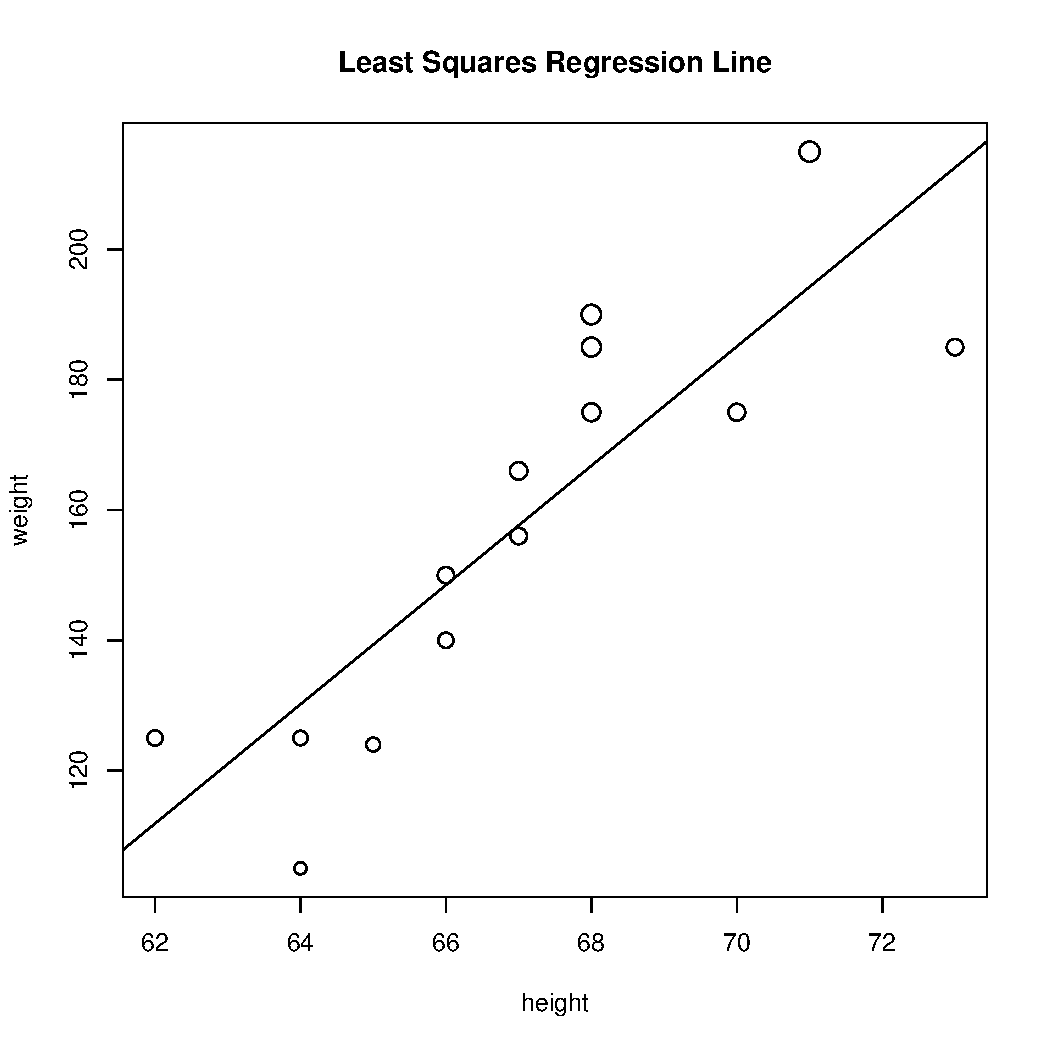
\includegraphics[width=\maxwidth]{figure/unnamed-chunk-3-1} 

\end{knitrout}
bmi is increasing with both weight and height.
\section{}

\begin{knitrout}
\definecolor{shadecolor}{rgb}{0.969, 0.969, 0.969}\color{fgcolor}\begin{kframe}
\begin{alltt}
\hlkwd{library}\hlstd{(rgl)}

\hlkwd{par3d}\hlstd{(}\hlkwc{params}\hlstd{=}\hlkwd{list}\hlstd{(}
  \hlkwc{windowRect}\hlstd{=}\hlkwd{c}\hlstd{(}\hlnum{100}\hlstd{,}\hlnum{100}\hlstd{,}\hlnum{600}\hlstd{,}\hlnum{600}\hlstd{)))}
\hlkwd{view3d}\hlstd{(} \hlkwc{theta} \hlstd{=} \hlnum{70}\hlstd{,} \hlkwc{phi} \hlstd{=} \hlnum{20}\hlstd{)}

\hlkwd{plot3d}\hlstd{(X[,}\hlnum{2}\hlstd{],X[,}\hlnum{3}\hlstd{],weight,}\hlstr{"height"}\hlstd{,}\hlstr{"bmi"}\hlstd{,}\hlstr{"weight"}\hlstd{,}
       \hlkwc{col}\hlstd{=}\hlstr{'darkgray'}\hlstd{)}
\hlkwd{planes3d}\hlstd{(betahat[}\hlnum{2}\hlstd{],betahat[}\hlnum{3}\hlstd{],}\hlkwc{c}\hlstd{=}\hlopt{-}\hlnum{1}\hlstd{,betahat[}\hlnum{1}\hlstd{],}\hlkwc{add}\hlstd{=}\hlnum{TRUE}\hlstd{,}
         \hlkwc{alpha}\hlstd{=}\hlnum{.5}\hlstd{,}\hlkwc{col}\hlstd{=}\hlstr{"lightblue"}\hlstd{)}

\hlcom{# Save pdf}
\hlkwd{rgl.postscript}\hlstd{(}\hlstr{"plot.pdf"}\hlstd{,}\hlstr{"pdf"}\hlstd{)}
\end{alltt}
\end{kframe}
\end{knitrout}
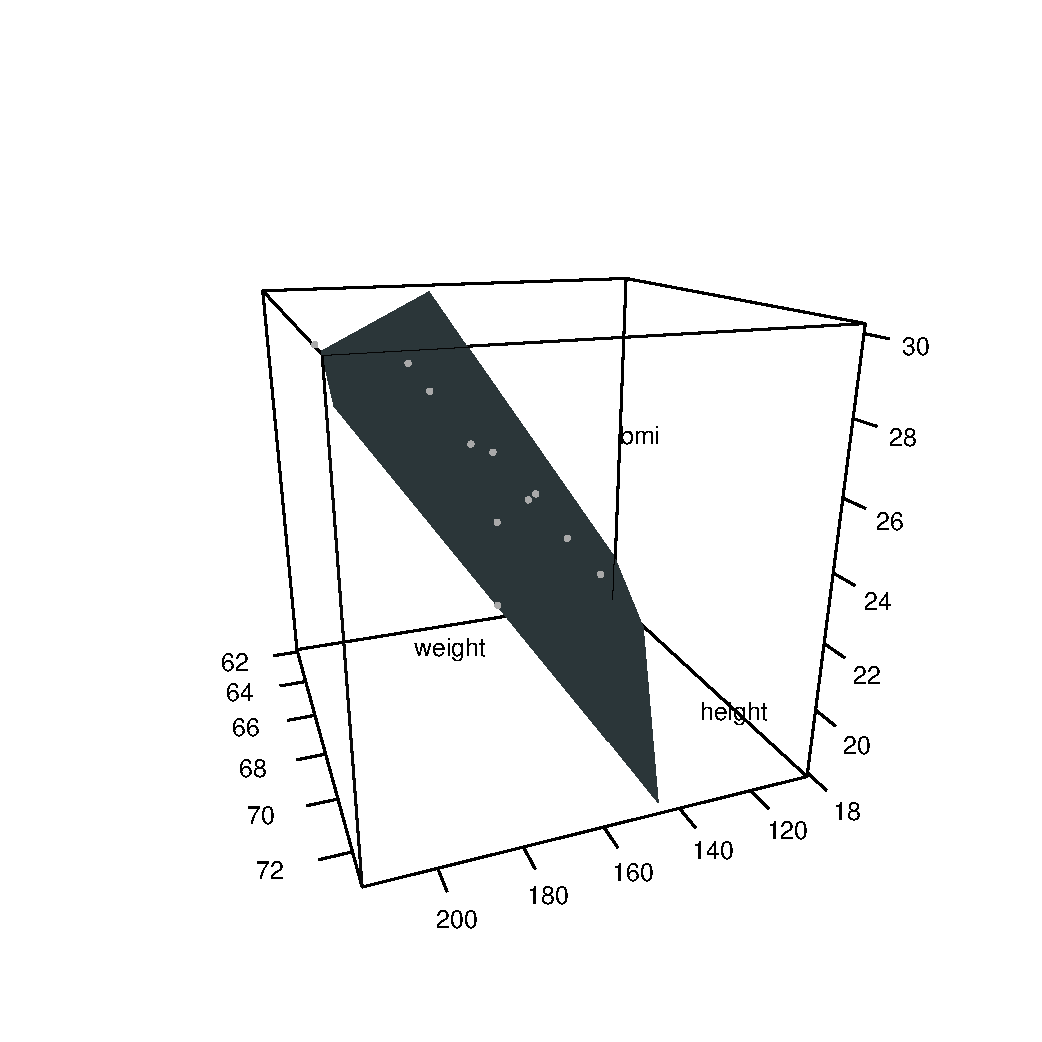
\includepdf{plot.pdf}

\section{}

\begin{knitrout}
\definecolor{shadecolor}{rgb}{0.969, 0.969, 0.969}\color{fgcolor}\begin{kframe}
\begin{alltt}
\hlstd{M} \hlkwb{=} \hlstd{X[,}\hlnum{1}\hlopt{:}\hlnum{2}\hlstd{]}
\hlstd{N} \hlkwb{=} \hlstd{X[,}\hlnum{3}\hlstd{]}
\hlstd{Y} \hlkwb{=} \hlstd{weight}

\hlcom{# step 1}
\hlstd{gamma_1} \hlkwb{=} \hlkwd{solve}\hlstd{(}\hlkwd{crossprod}\hlstd{(M,M),} \hlkwd{crossprod}\hlstd{(M,Y))}
\hlstd{gamma_1}
\end{alltt}
\begin{verbatim}
##                [,1]
## intercept -455.6660
## height       9.1537
\end{verbatim}
\begin{alltt}
\hlstd{f} \hlkwb{=} \hlstd{Y} \hlopt{-} \hlstd{M} \hlopt \hlstd{gamma_1}

\hlcom{# step 2}
\hlstd{gamma_2} \hlkwb{=} \hlkwd{solve}\hlstd{(}\hlkwd{crossprod}\hlstd{(M,M),} \hlkwd{crossprod}\hlstd{(M,N))}
\hlstd{gamma_2}
\end{alltt}
\begin{verbatim}
##                  [,1]
## intercept -23.0349135
## height      0.7098557
\end{verbatim}
\begin{alltt}
\hlstd{g} \hlkwb{=} \hlstd{N} \hlopt{-} \hlstd{M} \hlopt \hlstd{gamma_2}

\hlcom{# step 3}
\hlstd{gamma_3} \hlkwb{=} \hlkwd{sum}\hlstd{(f}\hlopt{*}\hlstd{g)}\hlopt{/}\hlkwd{sum}\hlstd{(g}\hlopt{*}\hlstd{g)}
\hlstd{gamma_3}
\end{alltt}
\begin{verbatim}
## [1] 6.308645
\end{verbatim}
\begin{alltt}
\hlstd{e} \hlkwb{=} \hlstd{f}\hlopt{-}\hlstd{g}\hlopt{*}\hlstd{gamma_3}

\hlcom{# step 4}
\hlstd{betahatBis} \hlkwb{=} \hlkwd{c}\hlstd{(gamma_1}\hlopt{-}\hlstd{gamma_2}\hlopt{*}\hlstd{gamma_3,gamma_3)}
\hlstd{betahatBis}
\end{alltt}
\begin{verbatim}
## [1] -310.346943    4.675473    6.308645
\end{verbatim}
\begin{alltt}
\hlcom{# Check validity }
\hlkwd{abs}\hlstd{(betahat}\hlopt{-}\hlstd{betahatBis)}
\end{alltt}
\begin{verbatim}
##                   [,1]
## intercept 6.082246e-12
## height    1.803002e-13
## bmi       2.522427e-13
\end{verbatim}
\end{kframe}
\end{knitrout}



\end{document}
